\documentclass[border=5mm,tikz]{standalone}
\usepackage{tikz}
\begin{document}

  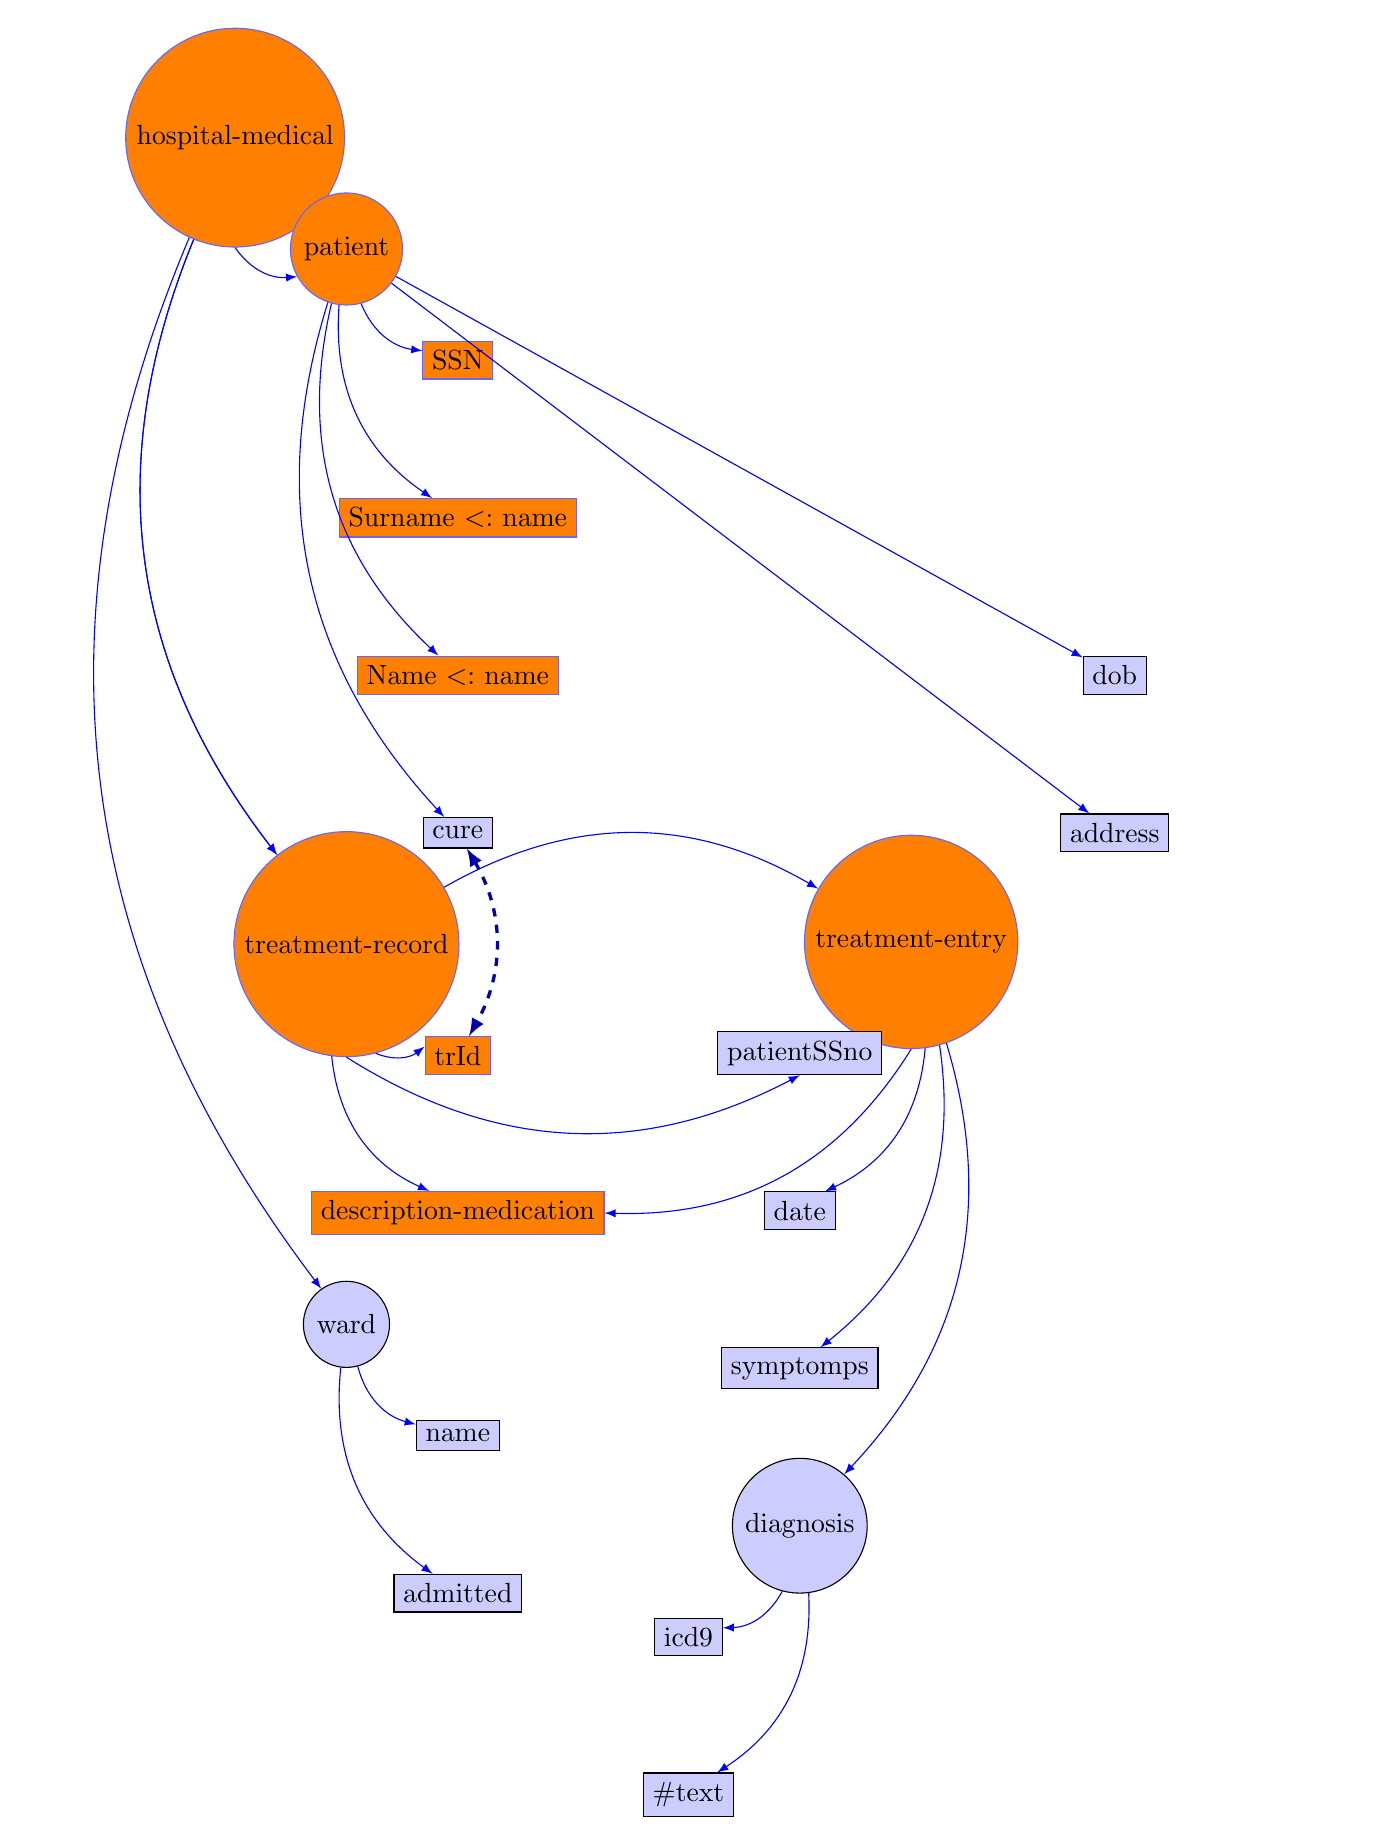
\begin{tikzpicture}[align=center,node distance=2cm]
	\node[circle,fill=orange,draw=blue!60] (lHospital) {hospital-medical};

	\node[circle,fill=orange,draw=blue!60, below right of=lHospital] (lPatient)  {patient};
		\path[-latex,blue] (lHospital.south) edge [bend right,above]  (lPatient);
		
		\node[rectangle,fill=orange,draw=blue!60, below right of=lPatient] (SSN)  {SSN};
			\path[-latex,blue] (lPatient) edge [bend right,above]  (SSN);
			
		\node[rectangle,fill=orange,draw=blue!60, below  of=SSN] (surname)  {Surname $<:$ name};
			\path[-latex,blue] (lPatient) edge [bend right,above]  (surname);
			
		\node[rectangle,fill=orange,draw=blue!60, below  of=surname] (name)  {Name $<:$ name};
			\path[-latex,blue] (lPatient) edge [bend right,above]  (name);
			
		\node[rectangle,fill=blue!20,draw, below  of=name] (cure)  {cure};
			\path[-latex,blue] (lPatient) edge [bend right,above]  (cure);
	
	\node[circle,fill=orange,draw=blue!60, below left of=cure] (lTreatment)  {treatment-record};
		\path[-latex,blue] (lHospital) edge [bend right,above]  (lTreatment);
		
	\node[circle,fill=orange,draw=blue!60, below left of=cure] (rEntry) at (10,-8.8) {treatment-entry};
		\path[-latex,blue] (lHospital) edge [bend right,above]  (lTreatment);
	
		\node[rectangle,fill=orange,draw=blue!60, below right of=lTreatment] (trId)  {trId};
			\path[-latex,blue] (lTreatment) edge [bend right,above]  (trId);
			
		\node[rectangle,fill=orange,draw=blue!60, below  of=trId] (description)  {description-medication};
			\path[-latex,blue] (lTreatment) edge [bend right,above]  (description);
			
	\node[circle,fill=blue!20,draw, below left of=description] (lWard)  {ward};
		\path[-latex,blue] (lHospital) edge [bend right,above]  (lWard);
		
		\node[rectangle,fill=blue!20,draw, below right of=lWard] (wname)  {name};
			\path[-latex,blue] (lWard) edge [bend right,above]  (wname);
		
		\node[rectangle,fill=blue!20,draw, below  of=wname] (admitted)  {admitted};
			\path[-latex,blue] (lWard) edge [bend right,above]  (admitted);
			
			
%    \foreach \ang/\lab/\User in {0/C/Carl,72/E/Eric,144/D/Dom} {
%      \node[rectangle,fill=blue!20,draw] (\lab) at ({\ang+17}:2){\User};
%    }
%    %\path[-latex,blue] (A) edge [above] node [blue] {fof} (B);
%   % \path[-latex,blue] (A) edge [above] node [blue] {fof} (C);
%    %\path[-latex,blue] (B) edge [above] node [blue] {fof} (D);
%    \path[-latex,blue] (E) edge [near end, below] node [blue] {fof} (D);
%    \path[-latex,blue] (E) edge [above] node [blue] {fof} (C);
%    \node[rectangle,fill=blue!20,draw] (F) at (19.5:4.14){Fred};
%    \node[rectangle,fill=blue!20,draw] (G) at (52.5:5){Greg};
%    \path[-latex,blue] (C) edge [above] node [blue] {fof} (F);
%    \path[-latex,blue] (F) edge [above] node [blue] {fof} (G);
%    \path[-latex,blue] (E) edge [above] node [blue] {fof} (G);
%    
%    \node[circle,fill=blue!20,draw] (2) at (0,0) {Apple};
%    \node[circle,fill=blue!20,draw] (1) at (0,4) {Microsoft};
%    \node[circle,fill=blue!20,draw] (3) at (2,2) {Pixar};
%    
%       % \draw[-latex,ultra thick] (A) --(1);
%       % \draw[-latex,ultra thick] (B) --(1);
%        \draw[-latex,ultra thick] (D) --(1);
%        
%              \draw[-latex,ultra thick] (D) --(2);
%              \draw[-latex,ultra thick] (C) --(2);
%              \draw[-latex,ultra thick] (E) --(2);
%
%   \draw[-latex,ultra thick] (E) --(3);
%   \draw[-latex,ultra thick] (F) --(3);
%   \draw[-latex,ultra thick] (G) --(3);


	\node (rMedical) at (14,0) {};
	
	\node[below left of=rMedical] (rPatient)  {};
		%\path[-latex,blue] (lHospital) edge [bend left,above]  (lPatient);
		
		\node[below left of=rPatient] (ssNo)  {};
			%\path[-latex,blue] (lPatient) edge [bend left,above]  (SSN);
			
		\node[below of=ssNo] (rName)  {};
			
		\node[rectangle,fill=blue!20,draw, below of=rName] (dob)  {dob};
			\path[-latex,blue] (lPatient) edge [above]  (dob);

		\node[rectangle,fill=blue!20,draw, below of=dob] (address)  {address};
			\path[-latex,blue] (lPatient) edge [above]  (address);
			
	%\node[ below right of=address] (rRecord)  {};
		%\path[-latex,blue] (lHospital) edge [bend left,above]  (lTreatment);
			
		%\node[ below  of=patientSSno] (rEntry2)  {};
			\path[-latex,blue] (lTreatment) edge [bend left,above]  (rEntry);
			
			
			
			
			\node[rectangle,fill=blue!20,draw, below left of=rEntry] (id)  {patientSSno};
				\path[-latex,blue] (lTreatment.south) edge [bend right,above]  (id.south);
				
			\node[rectangle,fill=blue!20,draw, below  of=id] (date)  {date};
				\path[-latex,blue] (rEntry) edge [bend left,above]  (date);
				
			\node[rectangle,fill=blue!20,draw, below  of=date] (symptomps)  {symptomps};
				\path[-latex,blue] (rEntry) edge [bend left,above]  (symptomps);
				
			\node[circle,fill=blue!20,draw, below  of=symptomps] (diagnosis)  {diagnosis};
				\path[-latex,blue] (rEntry) edge [bend left,above]  (diagnosis);
				
				\node[rectangle,fill=blue!20,draw, below left of=diagnosis] (icd9)  {icd9};
					\path[-latex,blue] (diagnosis) edge [bend left,above]  (icd9);
					
				\node[rectangle,fill=blue!20,draw, below  of=icd9] (text)  {\#text};
					\path[-latex,blue] (diagnosis) edge [bend left,above]  (text);
					
			%\node[rectangle,fill=blue!20,draw, below right of=text] (medication)  {medication};
				\path[-latex,blue] (rEntry.south) edge [bend left,above]  (description.east);
	
	
	%\path[latex-latex,green!70!black,very thick,dashed] () edge [above]  (rEntry);
	%\path[latex-latex,green!70!black,very thick,dashed] (lTreatment) edge [above]  (rRecord);
	%\path[latex-latex,green!70!black,very thick,dashed] (trId) edge [above]  (id);
	\path[latex-latex,blue!70!black,very thick,dashed] (cure) edge [bend left,above]  (trId);
  \end{tikzpicture}

\end{document}